% ============================================================
% 《借灯》项目文档 —— 主控文件
%
% 本文件只做两件事：加载配置、按顺序拼装各章节。
% 正文一个字都不写在这里，请编辑 chapters/ 下对应的章节文件。
%
% 编译：bash build.sh      （或 xelatex main.tex，需跑两遍以上）
% ============================================================

% !TeX program = xelatex
% 说明：本文档使用 ctex，必须用 XeLaTeX 编译，pdflatex 会失败。
% 这行是给 Overleaf 等编辑器看的；VS Code 已用全局 recipe 指定 xelatex。

\documentclass[UTF8, fontset=windows, 12pt, a4paper]{ctexrep}
\usepackage{graphicx}
% ============================================================
% tex/info.tex —— 项目元信息
%
% 封面、页眉、PDF 属性都从这里取值。
% 需要改动项目信息时只改这一个文件，不要散落在正文里。
% ============================================================

\newcommand{\ProjectName}{借灯}
\newcommand{\ProjectSubtitle}{一盏灯，照见一段被掩埋的真相}

\newcommand{\CourseName}{网站开发小学期}
\newcommand{\Instructor}{赵丰年}
\newcommand{\TeamName}{白灯客}
\newcommand{\TeamMembers}{罗晨菲、杨梦、于知让、高冰轩、卢正松}

\newcommand{\DocDate}{2026 年 9 月}
\newcommand{\DocVersion}{v1.0}
        % 项目元信息（项目名、组员、课程……）
% ============================================================
% tex/preamble.tex —— 全局排版设置
%
% 只负责"整份文档长什么样"：页面、颜色、章节标题格式、
% 代码样式、页眉页脚、超链接。
% 正文命令在 tex/commands.tex，正文内容在 chapters/。
% ============================================================

% ---------- 中文数字章号：一、二、……十一 ----------
% 自己定义而不依赖 ctex 的 \chinese / zhnumber，避免宏包版本差异导致编译失败。
\newcommand{\chapterlabel}{%
  \ifcase\value{chapter}\or
  一\or 二\or 三\or 四\or 五\or 六\or
  七\or 八\or 九\or 十\or 十一\or 十二\fi
}

% ---------- 页面尺寸与边距 ----------
\usepackage{geometry}
\geometry{
  a4paper,
  top=2.8cm, bottom=2.5cm,
  left=3.0cm, right=3.0cm,
}

\linespread{1.35}

% ---------- 图片与表格 ----------
\usepackage{graphicx}
\usepackage{booktabs}
\usepackage{tabularx}
\usepackage{array}
\usepackage{caption}

% 长表格：xltabular = tabularx 的自动列宽 X + longtable 的跨页断行。
% 用于行数多到一页放不下的表（如第二章的场景清单），
% 否则浮动体被推迟到下一页，小标题会和表格分家。
\usepackage{xltabular}
\setlength{\LTpre}{8pt}    % 表前距（默认偏大）
\setlength{\LTpost}{8pt}   % 表后距
\setlength{\LTcapwidth}{\linewidth}
\renewcommand{\arraystretch}{1.15}
\captionsetup{font=small, labelsep=quad, skip=6pt}

% 浮动体放置参数。默认值下，同一节里挨着的两张表很容易被 LaTeX 判定为
% "这一页放不下正文了"，于是单独排成一页浮动页，正文被推到前后两页，
% 中间留出半页空白（第三章的色板表与字体表、视频表与转场表都撞上过）。
% 放宽"一页能放几个浮动体"和"浮动体最多占多大比例"，让表和正文同页。
\setcounter{topnumber}{3}
\setcounter{bottomnumber}{2}
\setcounter{totalnumber}{4}
\renewcommand{\topfraction}{0.92}      % 顶部浮动体最多占版心的比例
\renewcommand{\bottomfraction}{0.85}
\renewcommand{\textfraction}{0.06}      % 一页至少留多少正文
\renewcommand{\floatpagefraction}{0.85} % 不到这个比例就不单独排浮动页

% ---------- 流程图 ----------
% 用 TikZ 画在图环境里，不依赖外部工具导出的图片：改节点文字不用重新画图，
% 编译出来是矢量，缩放不糊。arrows.meta 提供 -{Stealth} 这类箭头样式。
\usepackage{tikz}
\usetikzlibrary{arrows.meta, positioning}

% ---------- 颜色 ----------
\usepackage{xcolor}
\definecolor{nightblue}{RGB}{26,35,58}    % 夜色深蓝：标题主色
\definecolor{lampgold}{RGB}{201,146,42}   % 灯焰暖黄：强调色
\definecolor{papergray}{RGB}{248,248,246} % 纸张灰：代码底色

% ---------- 代码块 ----------
\usepackage{listings}
\lstset{
  basicstyle=\small\ttfamily,
  backgroundcolor=\color{papergray},
  commentstyle=\color{black!45},
  keywordstyle=\color{nightblue}\bfseries,
  stringstyle=\color{lampgold},
  numbers=left,
  numberstyle=\tiny\color{black!35},
  numbersep=8pt,
  frame=single,
  framerule=0.4pt,
  rulecolor=\color{black!15},
  breaklines=true,
  showstringspaces=false,
  tabsize=2,
  columns=flexible,
  keepspaces=true,
}

% ---------- 章节标题格式 ----------
\ctexset{
  chapter = {
    name       = {},
    number     = \chapterlabel,
    aftername  = {、},
    format     = \centering\Large\bfseries\color{nightblue},
    beforeskip = 1.0em,
    afterskip  = 1.8em,
    pagestyle  = fancy,
  },
  section = {
    format     = \large\bfseries\color{nightblue},
    aftername  = {\quad},
    beforeskip = 1.2em,
    afterskip  = 0.8em,
  },
  subsection = {
    format = \normalsize\bfseries\color{black!85},
  },
  subsubsection = {
    format = \normalsize\bfseries\color{black!75},
  },
}

% ---------- 目录里章号的分隔符 ----------
\usepackage{etoolbox}

% ctex 写入 .toc 时把章号与标题之间的分隔符硬编码成 \hspace{.3em}，
% 与标题行的「、」对不上，这里改掉。补丁失败会打印警告，不会被无声忽略。
\makeatletter
\AtBeginDocument{%
  \patchcmd{\CTEX@chapter@tocline}
    {\hspace{.3em}}
    {、}
    {}{\PackageWarning{project-report}{目录章号分隔符补丁未生效：TOC 里会显示成“一 标题”}}%
}
\makeatother

% ---------- 页眉页脚 ----------
\usepackage{fancyhdr}
\setlength{\headheight}{15pt}
\pagestyle{fancy}
\fancyhf{}
\fancyhead[L]{\small\color{black!50}\ProjectName · 项目文档}
\fancyhead[R]{\small\color{black!50}\leftmark}
\fancyfoot[C]{\small\thepage}
\renewcommand{\headrulewidth}{0.4pt}
\renewcommand{\footrulewidth}{0pt}

% 章首页沿用相同页眉页脚（否则章首页会退回朴素样式）
\fancypagestyle{plain}{
  \fancyhf{}
  \fancyhead[L]{\small\color{black!50}\ProjectName · 项目文档}
  \fancyhead[R]{\small\color{black!50}\leftmark}
  \fancyfoot[C]{\small\thepage}
  \renewcommand{\headrulewidth}{0.4pt}
  \renewcommand{\footrulewidth}{0pt}
}

% ---------- 超链接（必须最后加载）----------
\usepackage{hyperref}
\hypersetup{
  colorlinks        = true,
  linkcolor         = nightblue,
  citecolor         = lampgold,
  urlcolor          = lampgold,
  bookmarksnumbered = true,
  bookmarksopen     = true,
  pdftitle          = {\ProjectName 项目文档},
  pdfauthor         = {\TeamName},
}
    % 全局排版设置
% ============================================================
% tex/commands.tex —— 正文里反复使用的自定义命令
% ============================================================

% ---------- 待补充标记 ----------
% 编译出来是醒目的红色，防止"某章其实还空着"被无声放过。
% 定稿前全局搜索 \pending 确认已清空。
\newcommand{\pending}[1][待补充]{%
  {\color{red}\bfseries 【#1】}%
}

% ---------- 色块（第三章色板表用）----------
% 用法：\swatch{cBg}
% 在表格里直接画出颜色本身，省掉一张色板截图（截图里的色值会被屏幕和
% 压缩改掉，色块不会）。
%
% 块里必须 \phantom 占位，不能写 \colorbox{#1}{\rule{...}}：\rule 是用
% 当前文字色（黑）画的，会盖住底色，只漏出 \fboxsep 那圈彩边，看起来
% 就是一个黑心彩环。\phantom 只占尺寸不着色，底色才透得出来。
% 外面套一层 \fcolorbox 加细灰边，--lamp 这类浅色在纸上才有边界。
%
% 颜色必须先 \definecolor 起名再引用，不写 \swatch{#07090e}：tabularx
% 会把表体整段抓成宏，表体里裸的 # 会被当成参数号，报
% "Illegal parameter number in definition of \XC@@tmp"。
\definecolor{cBg}{HTML}{07090E}
\definecolor{cBgElevated}{HTML}{0D1118}
\definecolor{cLamp}{HTML}{F5F0E3}
\definecolor{cPaper}{HTML}{ECE7DC}
\definecolor{cPaperDim}{HTML}{CFC8B8}
\definecolor{cAccent}{HTML}{D8C6A4}
\definecolor{cAccentDeep}{HTML}{B89B6E}
\definecolor{cMist}{HTML}{8FB8CE}
\definecolor{cRain}{HTML}{5D7F9E}
\definecolor{cCinnabar}{HTML}{A6534A}
\definecolor{cDanger}{HTML}{C17A74}
\newcommand{\swatch}[1]{%
  {\setlength{\fboxsep}{0pt}\setlength{\fboxrule}{0.4pt}%
   \fcolorbox{black!35}{#1}{\phantom{\rule{1.7em}{1.05em}}}}%
}

% ---------- 插图 ----------
% 用法：\fig[宽度比例]{图片路径}{图注}{标签}
%   \fig[0.8]{figures/01-overview/cover.png}{游戏封面}{cover}
% 正文引用：图\ref{fig:cover}
% 宽度比例省略时默认 0.8；数值是相对版心宽度的比例。
\newcommand{\fig}[4][0.8]{%
  \begin{figure}[htbp]
    \centering
    \includegraphics[width=#1\linewidth]{#2}
    \caption{#3}
    \label{fig:#4}
  \end{figure}
}

% ---------- 截图占位 ----------
% 第七章的截图未到位时先用它顶上，文件本身不依赖任何图片，编译能过。
% 用法与 \fig 完全一致（后三个参数原样保留），图片就位后把 \figph 改成
% \fig、再把第二参数换成图片路径即可，其余不用动。
%   \figph[0.8]{入口页·封面首屏}{入口页封面}{entry}
% 第一个可选参数仍是宽度比例。框体高度固定为 0.45\linewidth：桌面图传
% 0.8 得到 16:9，手机竖版图传 0.22 得到接近真机的长宽比。
\newcommand{\figph}[4][0.8]{%
  \begin{figure}[htbp]
    \centering
    \setlength{\fboxsep}{5pt}%
    \fcolorbox{black!30}{black!4}{%
      \parbox[c][0.45\linewidth][c]{#1\linewidth}{%
        \centering\small\color{black!55}%
        {\color{red}\bfseries 待截图}\\[4pt] #2}}%
    \caption{#3}
    \label{fig:#4}
  \end{figure}
}
    % 正文自定义命令

\begin{document}

% ---------- 封面 ----------
% ============================================================
% tex/cover.tex —— 封面
% 所有文字取自 tex/info.tex，此处不要写死项目名或人名。
% ============================================================

\begin{titlepage}
\centering

\vspace*{2.5cm}

{\Huge\bfseries\color{nightblue} 《\ProjectName》\par}

\vspace{0.9cm}

{\large\color{lampgold}\ProjectSubtitle\par}

\vspace{2.2cm}

{\LARGE\bfseries 项目文档\par}

\vspace{1.2cm}

{\large\color{black!60}\DocVersion\par}

\vspace{2.5cm}

{\large
\renewcommand{\arraystretch}{1.7}
\begin{tabular}{r@{\quad}p{8cm}}
  \textbf{课程名称} & \CourseName \\
  \textbf{指导教师} & \Instructor \\
  \textbf{项目组}   & \TeamName \\
  \textbf{小组成员} & \TeamMembers \\
\end{tabular}\par}

\vfill

{\large \DocDate\par}

\vspace{1.5cm}

\end{titlepage}


% ---------- 目录 ----------
\tableofcontents
\clearpage

% ---------- 正文：按大纲顺序拼装 ----------
% ============================================================
% 第一章 · 项目概述
% 对应大纲：# 一、项目概述
% ============================================================

\chapter{项目概述}

\section{游戏简介}

\pending

\section{体验定位}

\pending

\section{项目目标分期与实现边界}

\pending

% ============================================================
% 第二章 · 游戏设计详解
% 对应大纲：# 二、游戏设计详解
%
% 本章体量最大，若单个文件超过约 500 行，建议改为
% 建立同名的 chapters/02-game-design/ 目录，内部按小节拆成
% 多个 .tex，再在本文件中用 \input{} 引入。
% ============================================================

\chapter{游戏设计详解}

\pending

% ============================================================
% 第三章 · 美学与用户体验
% 对应大纲：# 三、美学与用户体验
%
% 叙述口径：写我们最终要达到的视听标准与设计理由，不写当前完成度。
%
% 术语约定：
%   游戏名 = 《借灯》（\ProjectName）；组名 = 白灯客
%   白灯 = 故事里那盏没有火焰的纸灯笼，也是全篇唯一的暖光源
%
% 界面设计一节（站点地图 / 线框图 / 设计图）留标题，由组员自行补写。
% ============================================================

\chapter{美学与用户体验}

\section{视觉设计规范}

\subsection{整体风格}

《\ProjectName》的视觉只讲一个对比：冷夜里的那盏灯，基于强烈的冷暖对比进行设计。

故事里的白灯笼没有火焰，却在雨夜里泛着白光。它代表掩饰，在画面中被做成全篇唯一的暖光源。其余元素，雨、雾、废弃的矿区、没有窗的屋子，全部压在冷调里。玩家进入任何一个场景，视线都会先落到亮的那一点上。

这个对比同时解决了一个实际问题。全篇场景出自不同批次，祠堂在室内，矿井在地下，数据机房是现代的，如果各画各的，玩家每换一个地方都要重新适应。规范因此固定四样不变的东西：色板、雨、灯、字体。场景内容可以不同，这四样必须一致，玩家切换场景时感受到的是同一个雨夜里的不同地点。

\subsection{配色}

全站颜色收拢到一个变量文件里，其余样式表只引用变量名，不单独书写色值。这样做的目的是让配色一致性自动维持：修改一处底色，所有页面同步变化，不会出现主菜单与老宅场景相差三个色阶的情况。

\begin{table}[htbp]
\centering
\caption{全站色板}
\small
% Token 名写成 -{}-bg 而不是 --bg：xeCJK 下 \ttfamily 打开了 TeX 连字，
% 裸的 -- 会被排成破折号。
\begin{tabularx}{\linewidth}{@{}l l X@{}}
\toprule
分组 & 色块与 Token & 用途 \\
\midrule
冷底   & \swatch{cBg} \texttt{-{}-bg (\#07090e)}                & 页面最深底色，场景最暗处 \\
       & \swatch{cBgElevated} \texttt{-{}-bg-elevated (\#0d1118)} & 面板与卡片底 \\
       & \swatch{cBgElevated} \texttt{-{}-panel}                & 文本框与侧栏的半透明底 \\
\addlinespace
纸与暖金 & \swatch{cLamp} \texttt{-{}-lamp (\#f5f0e3)}           & 白灯的光，热点光晕与高光 \\
       & \swatch{cPaper} \texttt{-{}-paper (\#ece7dc)}          & 正文纸白 \\
       & \swatch{cPaperDim} \texttt{-{}-paper-dim (\#cfc8b8)}   & 次级文字、旧纸 \\
       & \swatch{cAccent} \texttt{-{}-accent (\#d8c6a4)}        & 强调暖金，木纹、旧物、描边 \\
       & \swatch{cAccentDeep} \texttt{-{}-accent-deep (\#b89b6e)} & 深金，按钮悬停态 \\
\addlinespace
冷点缀 & \swatch{cMist} \texttt{-{}-mist (\#8fb8ce)}            & 雾蓝，冷光与次级点缀 \\
       & \swatch{cRain} \texttt{-{}-rain (\#5d7f9e)}            & 雨蓝，雨丝与冷调 \\
\addlinespace
警示   & \swatch{cCinnabar} \texttt{-{}-cinnabar (\#a6534a)}    & 朱砂红，关键真相与门外的声音 \\
       & \swatch{cDanger} \texttt{-{}-danger (\#c17a74)}        & 错误与警示 \\
\bottomrule
\end{tabularx}
\end{table}

用色规则可以概括成一句：底色永远冷，强调永远暖。

朱砂红是使用限制最严的颜色，只允许出现在三处：关键真相线索、错误提示、门外那个叫名字的声音。一旦大面积使用，它就不再表示紧急，玩家对它的警觉也会随之消失。

两项可读性指标定为硬性要求：正文与背景的对比度不低于 4.5:1，最小的楷体字不小于 12px。探索区叠加在场景图上的标签必须垫一层深色半透明底，不能把浅色字直接压在亮背景上。场景图中存在高亮区域，浅色标签叠加其上会失去可读性。

\subsection{字体}

\begin{table}[htbp]
\centering
\caption{字体与字号阶梯}
\small
\begin{tabularx}{\linewidth}{@{}l l l X@{}}
\toprule
层级 & 字体 & 字号 / 行高 & 用途 \\
\midrule
标题 & 宋体 & 24px / 字距 0.18em & 游戏名、章节名、场景名 \\
正文 & 宋体 & 17--21px / 1.9 & 剧情正文、人物对白 \\
旁白与小字 & 楷体 & 12--15px / 1.6--1.8 & 说明性小字、旁白细节 \\
界面标签 & 无衬线 & 14px & 按钮、顶栏、系统提示 \\
\bottomrule
\end{tabularx}
\end{table}

宋体笔画清晰，适合长段落阅读，用于剧情正文和场景名。楷体接近手写，放在说明性小字上，与正文形成区分，避免提示文字打断阅读。按钮和顶栏需要快速识别，使用无衬线字体。

封面单独使用一套毛笔手写字体，全篇只在封面出现一次，重复使用会削弱它的辨识作用。

正文的 1.9 倍行高和标题 0.18em 的字距是依据中文排版特点设定的。中文没有词间空格，字号越大、字距越密，长句越容易读串行，行高和字距是替代空格的主要分隔手段。

\subsection{人物立绘}

立绘只有两个站位，左和右，分别落在画面两侧 5\% 的位置。哪个角色站哪边写在数据里，渲染层只读站位数值，不判断来的是谁。这样加一个人物不需要改渲染代码，改一个字段就够了。

立绘的作用是表示场景中有人在场，同一时刻只出现一个，站位的变化即表示说话人更换。

苏禾全篇不出正脸立绘，只以笔迹、照片和登记记录出现。这是因为，她的死要等到第二次汇合才揭晓，任何一张正脸立绘都会让玩家在她真正出场之前就先认出她。美术不必把每个角色都画出来，隐藏不该出现的角色同样是设计的一部分。

\subsection{美术原则}

场景图同时承担背景和线索载体的功能，美术有四条硬性要求。

\begin{enumerate}
  \item \textbf{光源统一。} 每个场景只设一处主白灯光源，位置随场景走：祠堂在门和梁上，村口在电杆和屋檐，老宅在门后。光晕半径约为场景短边的一半到七成。任何情况下不得遮住发光热点、线索和对白区。
  \item \textbf{冷暖不混。} 关键对象和热点不许埋在暖光晕里。玩家点哪一处、就看哪一处
  \item \textbf{画布与安全区统一。} 场景按 1280$\times$720 绘制，16:9，满屏不裁切。底部 600 到 720 一条留给阅读框和按钮，关键信息不往里放。
  \item \textbf{背景不许剧透。} 每张图交付前要过一遍：这张图有没有提前泄露某个人的结局、某一层身份的关系。有就改。
\end{enumerate}

这四条写进了场景交付模板，每张图由美术、剧情和前端三方逐项确认之后才能合入。氛围统一因此有了可以逐条核对的验收标准。

\subsection{动效规范}

日常动效控制到几乎不可察觉，只有三类。

雨丝垂直缓慢下移，透明度很低，不干扰阅读。白灯的光晕在 0.85 到 1 之间以约 2.5 秒的周期缓慢起伏，该效果只用在灯和发光热点上。场景切换统一使用 200 到 400 毫秒的淡入淡出，全篇不做变化。

限制强度的原因是：玩家要在这个界面上读三个小时的字，任何一处抢注意力的动效都会被反复看到几百遍。动效的作用是维持画面的活性，不是吸引玩家注意动效本身。

规范中另有一条硬性要求：动效不触发眩晕，不做大面积快速位移，并且尊重系统的减少动态效果设置。高强度的动态效果全部留给关键转场，见本章第四节。

\section{文字风格}

\subsection{整体调性}

全篇有一条硬性要求：游戏里出现的所有文字都要出自故事世界内部，不出现项目组直接对玩家说话的情况。

这一条在执行时比想象中容易破。V4 定稿时删改幅度最大的一批文案，问题几乎都出在这里。原文里有一句“恭喜你，成功解锁【陈家老宅】相关剧情”，句式上是系统提示，效果上把玩家从故事里拽了出来，让他在沉浸最深的时候意识到自己在操作一款游戏。同一批改写里还有一处“归档结论”，用文件摘要的语气替玩家把结论下完了。这两处最后都换掉了：前一句整句删除，后一句改由主角的独白提出，而且停在问句上。

判断标准可以总结成一句：结论由玩家得出，文本不替玩家下结论。

\subsection{用语}

写作时要求描述现场能直接看到、听到的东西。

改稿前有一段描述证据吻合的文案，用的是重合、证明、表明这一类词。这是文件摘要的口气，读起来像在审一份报告。改写之后变成了：纸已经很旧了，可撕口还是白的，是最近才撕开的。两句话说的是同一个判断，前一种写法要玩家自己翻译一遍，后一种写法直接把画面放到他眼前。

抽象概括会让玩家觉得自己在读材料，具体的形貌、声音、温度，才会让他觉得自己站在那个地方。

角色语言的个体差异在第二章已经展开过，这里只补充它对叙述层的要求：同一件事，村民用口语，小周用短句，主角用疑问句。叙述层不跟随任何一个人的语气，它始终是全篇最冷的那一层。

\subsection{氛围营造}

氛围的营造依靠信息的分寸，不依靠形容词。

全篇没有一句直接告诉玩家这里很吓人。与其写雨夜的村子很阴森，不如写纸上那道撕口还是白的。先给出一个具体的东西，再把它留给玩家自己去理解。

名牌制度也服务于这一点。旁白不出名牌，正文自己陈述，玩家读到的是一段没有来源的叙述；独白出名牌，那句话就被标记为主角自己的声音。两者在视觉上区分得很清楚，玩家始终知道一句话是谁说的，或者知道它没有来源。

情节里最沉重的细节，我们选择不做解释。父亲签下停止搜救那一段，处理方式是让玩家自己停下来，文本不跟任何评价。这种留白是刻意的，目的是把最后一步留给玩家自己完成。

\section{界面设计}

% 本节由组员补写，分三块：站点地图 / 线框图 / 设计图。
% 图片就位后用 \fig 插入，例如：
%   \fig[0.9]{figures/03-ux/sitemap.png}{站点地图}{sitemap}
% 站内页面清单（pages/ 目录，12 个）：
%   游戏主流程  pages/game.html
%   主菜单      pages/menu.html
%   登录 / 注册 pages/authorize/login.html、register.html
%   成就        pages/achievements/achievements.html
%   项目介绍    pages/about/project.html
%   制作组      pages/about/team.html
%   成员页 ×5   pages/about/members/{yu-zhirang,luo-chenfei,gao-bingxuan,
%               lu-zhengsong,yang-meng}.html

\subsection{站点地图}

\begin{figure}[htbp]
\centering
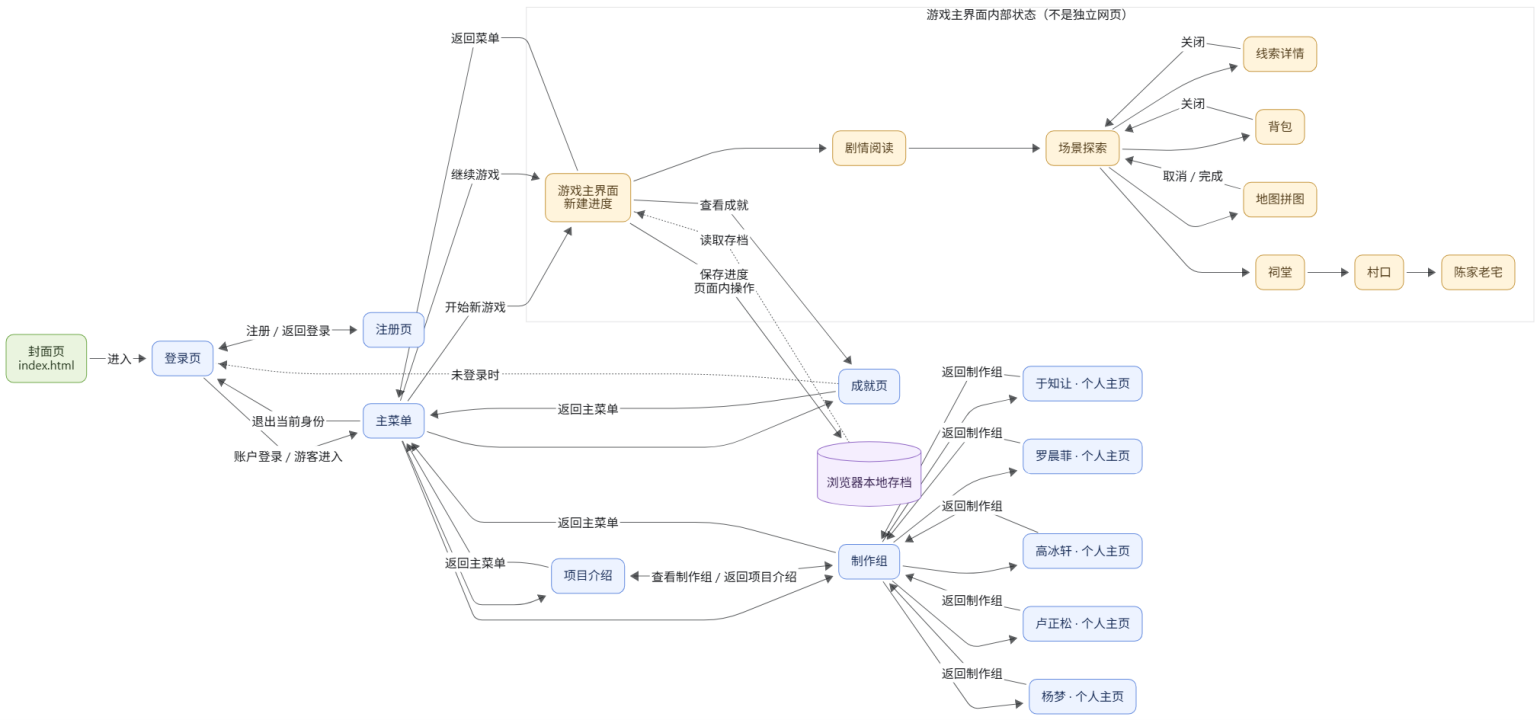
\includegraphics[width=0.9\textwidth]{figures/03-art-and-experience/locate.png}
\caption{站点地图结构}
\label{fig:locate}
\end{figure}

\subsection{线框图}

\pending

\subsection{设计图}

\begin{figure}[htbp]
\centering
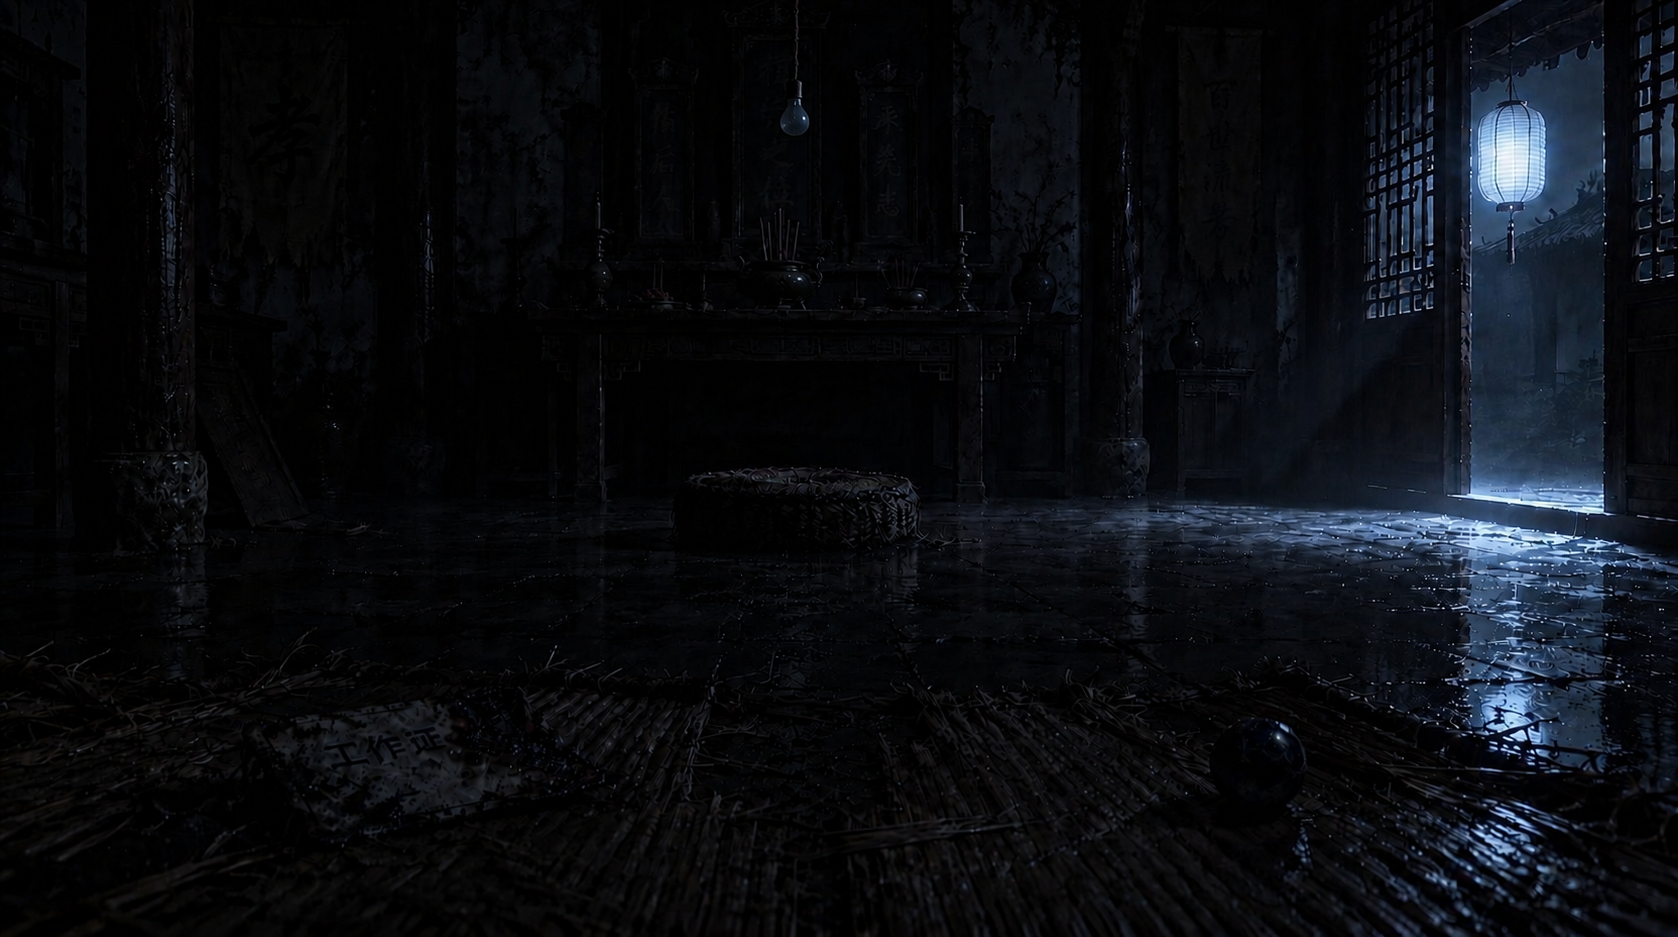
\includegraphics[width=0.9\textwidth]{figures/03-art-and-experience/lampUp.png}
\caption{祠堂灯亮设计}
\label{fig:lampUp}
\end{figure}

\begin{figure}[htbp]
\centering
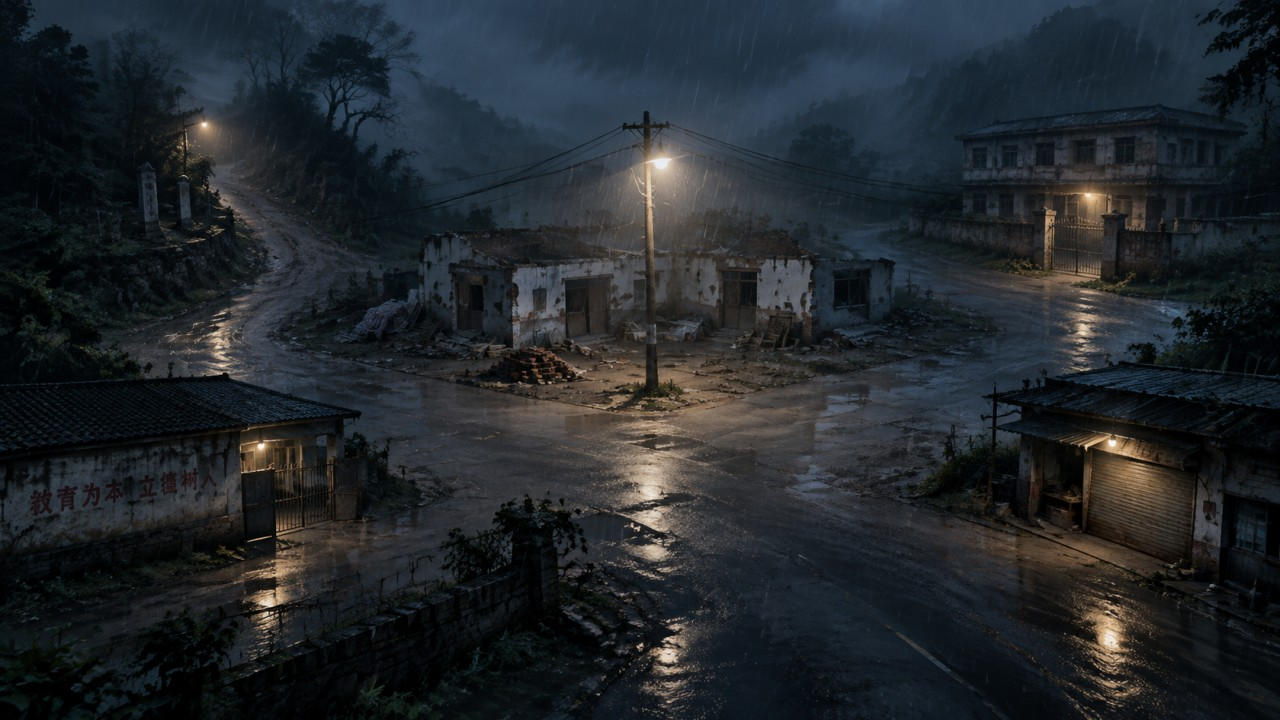
\includegraphics[width=0.9\textwidth]{figures/03-art-and-experience/outer-investigation-hub.jpg}
\caption{四条探索分支背景设计}
\label{fig:outer-investigation-hub}
\end{figure}



\section{恐怖美学设计}

\subsection{整体特点}

全篇的恐怖不使用惊吓手法。

惊吓的效果只持续几秒。我们采用的方式是持续的心理压抑：玩家玩到中段时意识到，自己刚才拆开的每一个装置，材质、颜色、声音，都来自主角小时候见过的东西。那一刻不产生惊吓反应，产生的是心理上的沉重感。

因此全篇没有突然出现的巨响，主要手法都带有一层铺垫：灯先闪两下才暗下去，声音先响画面再跟上，门外先叫一声名字，隔一拍玩家才听清那是谁。恐惧感来自预期落空的那半秒，与音量无关。

这套做法的核心是反差。玩家在前半段接受的是一套民俗禁忌的解释，中段被告知所有异象都是人为布置，此时本该放松。紧接着他会认出，布置所用的元素全部取材于主角的童年创伤，他把自己最怕的东西做成了恐吓他人的工具。恐惧的来源由外部转向人本身，并且落在玩家自己操控的这双手上。

\subsection{音效}

音效承担环境层，同时负责制造真假难辨的效果。

檐下的雨、排水渠里的水、广播里带电流杂音的童谣、远处传来的爆破回声，这几层声音持续存在。它们同时属于村庄的日常环境与恐吓装置的一部分。玩家在中段之前分不出哪一层是人为布置的，中段之后回头看，每一声都解释得通。让人不安的是玩家发现自己听了两个小时，却始终没有听出其中的区别。

背景音乐只有一条循环轨，音量控制在四成左右，切换页面时不重新起播。玩家在菜单、成就页和游戏之间来回切换，音乐不应中断。

浏览器的自动播放限制决定了第一次出声必须等待玩家的第一个操作。音频在玩家第一次点击或按键之后起播，在此之前保持静音，界面上另有一个常驻的静音开关。这项限制无法绕过，可以做的是不让它成为意外：玩家按下第一次鼠标时音乐正好响起，让它看起来是设计好的。

音频加载失败不能连带停止游戏。播放器返回失败码后，游戏降级为无声继续，控制台保留一条记录。玩家可以听不到背景音，但不能卡在黑屏前。

\subsection{视频}

过场视频用于静态画面无法交代的位置：人物的情绪转折、时间的跳跃、以及回忆片段的插入。这些位置用旁白叙述会拖慢节奏，因此交由视频承担。

全篇七段，序幕两段，五个结局各一段。

\begin{table}[htbp]
\centering
\caption{过场视频清单}
\small
\begin{tabularx}{\linewidth}{@{}l l X@{}}
\toprule
触发位置 & 素材 & 内容 \\
\midrule
序幕 · 白灯初现 & \texttt{light\_up} & 门外忽然亮起一盏灯 \\
序幕 · 祠堂断电 & \texttt{cut-off} & 祠堂内忽然断电 \\
结局一 · 交出证据 & \texttt{the\_ending} & 灯火照旧 \\
结局二 · 追逐失败 & \texttt{close\_well} & 井口又高一寸 \\
结局三 · 销毁全部 & \texttt{unnamed} & 姓名落尽 \\
结局四 · 选择性公开 & \texttt{after\_whitelamp} & 借来的黎明 \\
结局五 · 完整公开 & \texttt{no\_more\_lamp} & 此后无须借灯 \\
\bottomrule
\end{tabularx}
\end{table}

触发条件绑定在台词内容上，不绑定在剧情节点的编号上，读到对应句子才播放。这样处理在协作阶段省去很多返工：节点编号会随剧情改写而变动，如果视频绑定编号，每改一次文案就要重新核对七个编号，漏掉一个就会导致一段视频永远不播放。绑定文本之后，修改剧情不会漏掉视频，增加视频也不用改动剧情数据。每条视频只播一次。

\subsection{转场}

转场是全篇唯一使用高强度效果的位置。日常动效控制到几乎不可察觉，效果强度集中在下面这十一处。

三类基本手法，加一种抖动接闪黑的组合手法，共同点是都带有铺垫，没有一处是突然出现的。

\begin{table}[htbp]
\centering
\caption{转场手法}
\small
\begin{tabularx}{\linewidth}{@{}l l X@{}}
\toprule
手法 & 时长 & 过程 \\
\midrule
轻闪黑 & 0.9\,s & 快速压黑，短暂停顿后淡出 \\
窒息式闪黑 & 3.3\,s & 灯闪两下 $\rightarrow$ 黑幕以 550\,ms 漫上 $\rightarrow$ 黑暗中边缘红晕呼吸 1\,s $\rightarrow$ 以 1.5\,s 缓慢退出 \\
暴力抖动 & 0.65\,s & 位移从 18\,px 逐级递减到 0，叠加旋转与轻微模糊 \\
无信号花屏 & 2.1\,s & 随机噪点从画面某一点扩散到全屏，短暂停顿后收回到同一点并淡出 \\
抖动接黑 & 3.1\,s & 先抖动，120\,ms 后黑幕漫上，其余同窒息式 \\
\bottomrule
\end{tabularx}
\end{table}

窒息式闪黑中的两次灯光闪烁有明确作用。先铺垫再压黑，玩家在黑暗真正到来之前已有半秒的预感，恐惧感来自这半秒的预期落空，与黑暗本身无关。恢复阶段用 1.5 秒，比压黑慢了三倍，目的是让玩家在离开黑暗时多停留一会儿。

花屏的扩散和收束都从一个随机点开始，两次使用同一个点。收束速度慢于扩散，形成缩回原处的效果。

十一处触发同样全部绑定在台词上。一个监听器观察剧情文本的渲染结果，读到约定的句子就播放对应效果，剧情数据里不埋任何标记。这样处理的好处与视频一致：修改剧情不会漏掉转场，增加转场不需要改动剧情。

所有手法都绘制在场景层内部，与阅读区是两个独立的层。黑屏期间文本仍然存在，只是被遮住，恢复之后玩家可以接着读。全篇没有一处转场会顶掉正在显示的文字，也没有一处会接管鼠标。恐怖效果可以打断节奏，不打断操作。

% ============================================================
% 第四章 · 技术方案与质量保证
% 对应大纲：# 四、技术方案与质量保证
%
% 本章含代码片段，用 lstlisting 环境排版：
%   \begin{lstlisting}[language=JavaScript, caption={...}, label={lst:xxx}]
%   ...
%   \end{lstlisting}
% ============================================================

\chapter{技术方案与质量保证}

\pending

% ============================================================
% 第五章 · 项目管理与进度
% 对应大纲：# 五、项目管理与进度
% ============================================================

\chapter{项目管理与进度}

\pending

% ============================================================
% 第六章 · 测试与回帖情况总结
% 对应大纲：# 六、测试与回帖情况总结
% ============================================================

\chapter{测试与回帖情况总结}

\pending

% ============================================================
% 第七章 · 最终显示效果
% 对应大纲：# 七、最终显示效果
%
% 本章是成品展示章，以图为主、文字为辅，12 张图，按玩家的实际游玩
% 顺序排列：进入与开场 → 剧情与探索 → 玩法与终局 → 系统与视听。
% 排列依据是游玩顺序而不是功能模块：这 12 张连着看一遍等于把游戏走一遍。
%
% 取舍口径：图控制在 12 张以内，被砍掉的界面由正文文字补上（例如四个
% 小游戏只放一张图，另外三个在导语里点名）。删图不等于删信息。
%
% 图片放 figures/07-final-showcase/，命名见 figures/README.md
% （全小写英文 + 连字符）。
%
% 截图未到位时用 \figph 占位（定义在 tex/commands.tex），占位框不依赖
% 任何图片文件，编译能过。图片就位后把 \figph 改成 \fig、把第二个参数
% 换成图片路径，后三个参数原样保留。占位框里那行小字是给截图的人看的
% 操作说明，换成 \fig 之后自然消失；图注是永久的，已按最终效果写好。
%
% ---------- 12 张截图 ----------
%   7.1  入口页首屏 / 祠堂首屏
%   7.2  人物对白与立绘 / 村口 / 陈家老宅 / 线索详情卡
%   7.3  逃离数据机房 / 证据处置界面 / 五个结局拼图
%   7.4  成就页 / 移动端主游戏页 / 五种转场手法拼图
% 两张需要自己拼图：五个结局的画面拼成一张，五种转场的过程帧拼成一张。
%
% 被砍掉、想加回来时按顺序优先补这几张：制作组页（团队展示）、主菜单、
% 背包（物品与证物两个页签）、序幕视频「白灯初现」的截帧、项目介绍页、
% 另外三个小游戏、注册与登录页、18 个场景的缩略图总览。
%
% ---------- 名称以代码与 V3 文档为准，不用描述性说法 ----------
% 五个结局的正式名称是《共犯的终点》《封井之人》《无名者》《白灯之后》
% 《不再借灯》，出自 docs/docs-v3/V3剧情Node推进.md 与代码里的
% ending-* 节点。报告此前只用「交出证据」「销毁全部」这类触发条件指代
% 它们，现已按正式名统一到第一、二、三、七章。
% 四个小游戏在界面上的标题是「复原手绘地图」「拆解控制室网络」
% 「还原矿井路线」「逃离数据机房」，见 v3-minigame-gateway.js 的注册表。
% 第二章的「拆鬼」「路线解谜」是设计阶段的叫法，不是玩家看到的标题，
% 现已统一。各人个人总结里的措辞是本人原文，未改动。
% ============================================================

\chapter{最终显示效果}

本章按玩家的实际游玩顺序排列成品截图：从入口页进入，经序章、探索与四个小游戏，走到五个结局，最后是系统页面与多端适配。这 12 张连着看一遍，等于把《\ProjectName》走了一遍。

前面几章分别交代了设计规范、剧情结构与技术实现，本章只呈现跑起来之后的样子。截图均在正式版本上取得，不含原型稿与线框图。

\section{进入与开场}

玩家从入口页进入，经登录或游客通道到主菜单，再走进祠堂，游戏正式开始。这一节的两张图分别是全篇第一印象与第一幕。

入口页是全篇唯一使用毛笔手写字体的位置。冷调雨幕压满整屏，白灯是画面上唯一的暖光源，第三章定下的冷暖对比在这里第一次出现。

% 【必】
\figph[0.85]{入口页首屏：整屏雨幕 + 白灯 + 毛笔标题 + 「进入」按钮。浏览器全屏截图，不要带上书签栏和地址栏}{入口页首屏}{entry}

祠堂是序章的全部场景。主角从地上醒来，身上只有三件物品，旁边有一个自称小周的年轻人。这一屏同时是场景层、阅读层与对话框的第一次合流。

% 【必】
\figph[0.85]{祠堂首屏：主角醒来。截白灯亮起后的那一屏（祠堂有三张背景图：只有灯泡、灯泡与灯笼都亮、只有白灯笼），画面里要有小周和几处可点的热点}{祠堂首屏}{prologue-hall}

\section{剧情与探索}

剧情文本分旁白、独白与角色对白三层，渲染上靠名牌区分：旁白不出名牌，独白出名牌，玩家始终知道一句话是谁说的，或者知道它没有来源。立绘只有左右两个站位，站位变化即表示说话人更换。

% 【必】
\figph[0.85]{人物对白：带立绘的一屏，角色站在画面左侧或右侧，名牌与正文分行显示}{人物对白与立绘}{dialogue-npc}

探索以整张场景图作交互载体，全篇 18 个场景，覆盖村庄中枢、三条身份线、三处玩法场景和五个结局画面。场景里可调查的对象一律做成热点，调查后留下痕迹或标记为已调查。下面两张是其中的两个地址：村口是唯一的中枢，玩家在这里反复出入，把三条线的进度带回同一个地方；陈家老宅是陈晋年线的第一站，也是全篇第一处门后主光源。

% 【必】
\figph[0.85]{村口：中枢场景，画面上有多个可点热点。截玩家刚到这里、还没有调查过的状态}{村口·村庄中枢}{scene-village}

% 【必】
\figph[0.85]{陈家老宅：用刻名钥匙开门后的内景，带门后主光源}{陈家老宅}{scene-chen-house}

调查得到的物证进入背包，线索独立成页。玩家拿到的是物证，理解的是线索，证据链由线索之间互相印证构成。

% 【必】
\figph[0.85]{线索详情卡：点开一条关键线索后的卡片，朱砂红只出现在关键真相上}{线索详情卡}{clue-card}

\section{玩法与终局}

四个小游戏分别嵌在剧情节点上，玩完把结果回写给剧情模块，由剧情模块决定后续走向。复原手绘地图在村口，玩家从三名村民处取得碎片拼成村庄图；拆解控制室网络在广播室，逆向追踪童谣、白灯与湿脚印三类人工装置；还原矿井路线在旧矿井，从排水洞绕过封堵进入竖井；逃离数据机房是终局的俯视追逐，躲避小周的追捕、收集三份证据并撤离。下面这张是第四个，它在其中操作要素最全。

% 【必】
\figph[0.85]{逃离数据机房：俯视视角的追逐场面，画面里要有生命值、三份证据的收集进度和追捕者小周}{逃离数据机房与生命值}{minigame-chase}

终局最后一步不交给对话，而是给玩家一个证据处置界面。三个选项分别处理手里的材料：销毁全部证据、以白灯客的名义选择性公开、完整公开。加上对峙时的交出证据与追逐失败，全篇共五个稳定结局，每个结局配一段过场视频。

% 【必】
\figph[0.85]{证据处置界面：村口场景上的三个处置选项，是整个游戏的最终抉择}{证据处置界面}{evidence-disposition}

% 【必】需要自己拼图：五张结局画面横排拼成一张（或两行，上二下三）
\figph[0.85]{五个结局的画面拼成一张，从左到右依次是《共犯的终点》（交出证据）、《封井之人》（追逐失败）、《无名者》（销毁全部）、《白灯之后》（选择性公开）、《不再借灯》（完整公开）。需要自己拼图}{五个结局}{endings}

\section{系统与视听}

主菜单、成就页与成员页在主线之外，玩家中途可以随时返回。成就页收录 14 条成就，按剧情推进分成调查札记、灯下真相、终局余烬三组；五条结局成就被标记为隐藏条目，未解锁时只显示未明之章配合罗马数字序号，不渲染描述文案。

% 【必】
\figph[0.85]{成就页「雨夜留痕」：顶部解锁进度与进度条，下面是三组共 14 张卡片。截已解锁与未解锁混合的一屏}{成就页}{achievements}

全站按窄屏重排，热点与阅读框在 390 像素宽下依然可点可读。

% 【必】
\figph[0.22]{手机端竖版主游戏页：窄屏下的场景、阅读框与底部操作栏。用真机或开发者工具的手机模式截}{移动端主游戏页}{mobile-game}

转场是全篇唯一使用高强度效果的位置，共十一处，分五种手法：轻闪黑、窒息式闪黑、暴力抖动、无信号花屏、抖动接黑。日常动效压到几乎不可察觉，效果强度集中在这里。

% 【必】需要自己拼图：五种手法各取开始、高潮、结束三帧，横排五行
\figph[0.85]{五种转场各取过程帧拼成一张，每种取开始、高潮、结束三帧。窒息式闪黑与无信号花屏最出效果，至少这两种要拼进去}{五种转场手法}{transition-frames}

% ============================================================
% 第八章 · 小组总结
% 对应大纲：# 八、小组总结
% ============================================================

\chapter{小组总结}


9.1 项目开发全景复盘：从 0 到 1 的协作落地
在“程序设计与制作”课程大作业的驱动下，我们“六个基米哈一天”小组以《第
五人格》为 IP 原型，耗时三周完成网页小游戏《第五人格：推演终幕》的开发。项目以
“求生者剧情推演 + 监管者卡牌战斗”为核心玩法，涵盖剧情系统、战斗系统、存档系
统、地图交互等六大核心模块，最终交付包含 3 万字剧情、17 个人物档案、2 张可切换
地图、1 个修机小游戏及豆瓣电影 / 中华美食两个附属网站的完整成果。回顾开发全流
程，我们以 “每日会议为协作枢纽、分工互补为推进引擎、问题共解为突破关键”，实
现了从需求拆解到功能落地的高效推进。
9.1.1 第一周：框架搭建与基础攻坚（8.24-8.30）
项目启动阶段，我们聚焦 “定方向、搭框架、破初障”三大目标。8 月 24 日 - 25
日，组长赵硕涵牵头完成组队与方向决策，组织成员学习项目 PPT 后，经线下会议投票
确定开发“《第五人格》IP 二创交互游戏”，明确“剧情 + 战斗”双核心玩法；房金衡作
为剧情与战斗策划，整合成员创意形成第一版游戏大纲，规划“序章 + 四章主线”剧情
结构，定义“求生者推演（剧情向）+ 监管者战斗（卡牌向）”的核心循环；梁思齐、刘
雨桐、潘治鑫组成技术组，同步启动前端基础学习，王宇豪则单美术线推进，搭建像素
素材库。8 月 26 日 - 30 日，各模块进入基础开发阶段。技术组方面，梁思齐从前端三件
套入门，克服 CSS 语法误区（误写 tiles 类后改用 button 标签），完成登录界面与角色
移动类初步开发；刘雨桐聚焦成就系统，参考往届“肖申克”“瑞雪”等作品，拆解出
“Achievements.json 配置表 + AchievementManager 管理逻辑 + 弹窗 UI”的模块架构，
同步编写剧情对话界面；潘治鑫则钻研 localStorage 存储逻辑，为存档系统奠定基础。
剧情与战斗组方面，房金衡完成序章“初入庄园”剧本及第一章前两幕剧情，同时设计
战斗系统基础规则，定义 90 点初始生命值、2 点行动点的玩家参数，规划普通攻击、利
剑之刺等 12 类基础卡牌。美术组方面，王宇豪从零学习 Tiled Map Editor 与 Aseprite，完
成首个测试地图与主角像素小人初稿，解决素材风格不统一问题。此阶段，我们遭遇首
个技术难关——CORS 协议跨域问题。8 月 29 日，梁思齐、潘治鑫在调试地图切换与存
档加载时，发现直接打开 HTML 文件无法获取数据，经每日会议集体排查，最终参考往
届方案，通过 Python HTTP 服务器与 Live Server 插件双路径解决，同时总结出“避免绝
对路径、统一相对路径调用”的开发规范，为后续模块协作扫清障碍。
9.1.2 第二周：功能深化与协同突破（8.31-9.6）
进入核心开发阶段，我们以 “模块协同、问题共解”为核心，推动项目从“能用”
向“好用”升级。技术组实现多系统联动：梁思齐优化角色移动逻辑，修复“对话未完
成关闭后状态异常”“空气墙不精准”等 5 类 Bug，同时创新性地用 Web Audio API 将
地图钢琴改造为可交互小游戏，解决“Click Noise”杂音问题；刘雨桐重构剧情系统架
构，将 20 个场景剧情拆分至独立 JS 文件，通过 scriptEngine.js 统一接口，解决浏览
器加载限制（加入 datamanager 与 UCL 参数加载函数）；潘治鑫则分离成就与存档系
42
项目计划
统（避免前期耦合导致的维护难题），新增自动存档功能，实现“剧情跳转后角色位置
与背包状态无损恢复”。剧情与战斗组实现内容扩容：房金衡完成第一章收尾（厂长剧
情）与第二章审核，同步优化战斗系统，为监管者新增特色机制（如红夫人“重生”、蜘
蛛“蛛网反伤”），调整卡牌数值避免流派失衡；同时拓展附属项目，耗时 10 余小时用
Python（requests+lxml）爬取豆瓣电影 Top250 数据，突破反爬限制（设置 1 秒延迟、伪
造 headers），将电影名称、评分、海报等信息以 JSON 格式存储，完成电影欣赏网站开
发。美术组则推进地图迭代：王宇豪完成地下室地图第二版，优化房间布局（划分图书
区、药水区），通过 GIMP 缩放处理 16×16 与 32×32 素材比例问题，同时绘制带感叹号
的交互贴图，提升场景引导性。此阶段的关键突破在于 “跨模块协作机制”的建立。9
月 2 日，梁思齐在开发钢琴小游戏时，发现 iframe 与角色移动的鼠标聚焦冲突，经与王
宇豪（美工）、潘治鑫（存档）召开专项会议，最终实现“点击游戏区域控制小游戏、点
击下方控制角色”的分层交互逻辑；9 月 4 日，刘雨桐因数学建模竞赛请假前，提前完
成剧情系统文档梳理，确保潘治鑫能顺利对接存档接口，体现“无缝交接”的协作意识。
9.1.3 第三周：整合优化与成果交付（9.7-9.13）
收尾阶段，我们聚焦 “全流程测试、细节优化、成果整合”，确保项目符合课程交
付标准。技术组完成系统闭环：梁思齐解决战斗系统与存档的数据断联问题（通过日志
追踪定位参数传递时机错误），实现“战斗胜利后自动触发剧情、失败后重置状态”的
完整流程；潘治鑫开发修机小游戏，设计“校准进度条 + 钥匙解锁门”的地图衔接逻辑，
同时完成成就系统与结局的联动（Boss 战胜利触发“欧律狄刻”成就，失败触发“故事
的最后”成就）；刘雨桐则完成角色档案系统开发，通过 localStorage 实现“账号级解
锁状态存储”，同步导入全部 3 万字剧情，解决文件命名格式错误（如“1.jpg”误判为二
进制文件）。剧情与美术组完成内容收尾：房金衡撰写第四章双结局（“精神清醒”“永
坠混沌”），补充 17 个人物档案（含生日、特质、背景故事），同时调整战斗数值（如
作曲家“音韵”被动技能改为“回合开始抽 1 张牌”）；王宇豪则对地下室地图进行像
素级优化，为关键道具（实验笔记）添加 Aseprite 发光动画，校准所有碰撞框，确保场
景交互无死角。最终交付阶段，我们建立 “模块测试 - 交叉验收 - 整体联调”的三级质
检体系：赵硕涵统筹全流程测试，重点验证地图切换、存档加载、成就触发等关键路径；
各成员交叉测试非负责模块（如梁思齐测试剧情跳转、王宇豪测试战斗 UI），最终解决
“非 Live Server 环境钥匙获取异常”“结局页面音效不同步”等 8 类遗留问题，确保项目
稳定运行。
9.2 技术难关攻克：从“卡壳”到“破局”的能力跃迁
三周开发中，我们遭遇的技术挑战不仅是“问题清单”，更是团队技术认知与协作
能力升级的“催化剂”。每一次难关的突破，都伴随开发规范的完善与技术思维的深化。
9.2.1 跨域与资源加载：从“被动规避”到“主动规范”
CORS 协议与浏览器资源加载限制是项目初期最棘手的问题。8 月 29 日，梁思齐
在调试地图矩阵（用数字标记交互区域）时，发现直接打开 HTML 文件无法读取 JS 配
43
项目计划
置，控制台报错“Access to script at ’file:///...’ from origin ’null’ has been blocked by CORS
policy”；同期，潘治鑫的存档系统也出现“localStorage 数据无法跨页面共享”的问题。
初期，我们尝试修改文件路径、改用绝对路径调用，均以失败告终。在 8 月 29 日晚间
会议中，我们转变思路：先调研往届解决方案（发现“瑞雪”项目用 Python HTTP 服务
器启动），再分工测试不同方案——潘治鑫尝试用 Python 的 http.server 模块（命令
“python -m http.server 8000”），成功解决跨域问题；梁思齐则测试 Live Server 插
件，发现能自动处理资源加载。但新问题随之而来：不同成员使用不同启动方式，导致
代码路径调用混乱。为彻底解决此问题，我们共同制定 “资源调用三规范”：一是所有
文件统一使用相对路径；二是建立“assets”目录分类管理 JS、CSS、图片资源；三是在
readme 文档中明确“Python HTTP 服务器与 Live Server 双启动方式”的操作步骤。此规
范不仅解决了当前问题，更避免了后续多模块协作时的路径冲突，体现 “问题解决 - 规
范沉淀”的技术思维升级。
9.2.2 多系统联动：从“各自为战”到“接口协同”
随着模块增多，“系统间数据同步”成为新挑战。9 月 11 日，梁思齐在对接战斗系
统与地图主系统时，发现战斗结果无法回传至主游戏，导致玩家完成战斗后卡在结算界
面。经排查，问题根源在于：战斗系统的结果参数仅在本地存储，未通过存档接口同步
至主游戏的状态；同时，主游戏未监听战斗页面的关闭事件，无法主动拉取最新数据。
针对此问题，我们成立专项攻坚小组（梁思齐、潘治鑫、房金衡），通过三次短时会议
确定解决方案：一是在战斗系统的“战斗结束”函数中，新增调用存档接口的逻辑；二
是主游戏页面添加“onmessage”监听，接收战斗页面的关闭通知后，拉取最新数据；三
是定义统一的 URL 参数格式，确保参数传递无歧义。此次攻关让我们深刻认识到 “接
口设计先行”的重要性。此后，我们在新增模块前，都会先在每日会议中确定接口参数，
避免后期返工。这种 “先定义接口、再开发功能”的思路，使后续修机小游戏与地图门
解锁的对接仅用 2 小时完成，效率提升 60%。
9.2.3 像素美术与技术适配：从“风格割裂”到“视觉统一”
美术与技术的适配问题贯穿开发全程。王宇豪作为美工，初期面临“素材风格不统
一”“像素比例失调”两大难题。为解决这些问题，我们建立 “美术 - 技术协同机制”：
一是素材标准统一，王宇豪明确“所有素材采用 32×32 像素、统一暗色调”，并用 GIMP
批量处理；二是交互区域可视化，梁思齐在 Canvas 绘制时，为可交互物件添加半透明红
色边框（测试模式下显示），方便王宇豪校准美术位置；三是效果迭代反馈，王宇豪为
实验笔记添加发光动画后，梁思齐同步调整触发范围，确保玩家能清晰感知交互点。最
终，地下室地图的视觉与技术适配效果显著：场景风格统一，交互准确率达 100%。此
次协作也让我们明白：美术不仅是“视觉装饰”，更是 “交互引导”——王宇豪后期为
关键道具添加的发光动画，使玩家找到实验笔记的平均时间从 2 分钟缩短至 30 秒，极
大提升游戏体验。
44
项目计划
9.3 协作认知升级：从“分工”到“共生”的团队蜕变
三周开发不仅是项目落地的过程，更是团队协作认知从“简单分工”向“深度共生”
跃迁的过程。我们深刻体会到：优秀的团队不是“各做各的”，而是“彼此支撑、互为补
充”。
9.3.1 每日会议：从“进度同步”到“问题共治”
我们坚持的“每日 19 点线上会议”，是团队协作的 “核心枢纽”。会议初期以“各
自说进度”为主，效率较低；后改革为 “问题优先”模式——每次会议先聚焦 3 个核心
问题，再同步进度、分配任务。这一改革带来显著变化：针对 CORS 跨域问题，会议仅
用 40 分钟就确定解决方案；讨论战斗难度梯度时，技术、策划、美术共同形成“章节 -
角色 - 数值 - 视觉”四维联动的难度设计。改革后的会议解决问题效率提升 150%。更重
要的是，每日会议培养了 “责任共担”的意识。这种“补位不缺位”的协作，让项目在
成员有临时任务时仍能高效推进。
9.3.2 分工与补位：从“固定角色”到“动态支撑”
项目初期，我们按“技术、策划、美术”划分固定角色，但发现“绝对分工”无法
应对复杂需求。为此，我们转向 “核心角色 + 动态补位”的模式：每个成员有明确核心
职责，但同时需掌握其他领域的基础技能，以便在团队需要时补位。这种模式成效显著：
潘治鑫（核心存档）协助优化移动逻辑，用“状态机”思路重构代码；王宇豪（核心美术）
学习基础 HTML/CSS，协助优化页面排版，使响应式适配率从 70% 提升至 100%。“动
态补位”不仅提升了项目效率，更让每个成员看到 “自身工作的价值关联”，形成良性
协作循环。
9.3.3 冲突与共识：从“意见分歧”到“最优解共建”
开发中并非毫无冲突，而是通过“理性讨论、数据支撑”将冲突转化为“共识升级”
的契机。关于“战斗系统是否需要难度梯度”的分歧，我们采取 “数据验证 + 最小原
型”的方案：房金衡计算战斗回合数，梁思齐快速制作“配置表原型”，最终团队达成共
识——采用“配置表 + 动态加载”方案，既实现难度梯度，又避免代码冗余。此次冲突
让我们建立 “冲突解决三原则”：一是不回避分歧；二是用数据说话；三是做最小原型。
这一原则确保团队决策始终基于“可行性”与“玩家体验”，而非个人偏好。
9.4 项目开发认知：从“功能堆砌”到“用户体验”的思维转变
三周开发让我们对“游戏开发”的认知实现从“技术驱动”到“用户为中心”的深
刻转变。我们逐渐明白：优秀的游戏不仅是“功能的集合”，更是 “体验的闭环”。
9.4.1 从“实现功能”到“优化体验”：细节决定成败
初期，我们更关注“功能是否实现”，而忽略“体验是否流畅”。例如，角色移动在高
刷新率电脑上过快，成就弹窗会遮挡战斗界面。针对测试反馈，我们启动 “体验优化专
项”：梁思齐用“requestAnimationFrame”替代固定时间间隔，并添加移动加速度，使
移动手感更佳；刘雨桐优化成就弹窗，新增“战斗中延迟显示”逻辑，并调整位置至右
45
项目计划
下角。体验优化后的效果显著：第二次测试中，玩家对“移动流畅度”的满意度从 40%
提升至 90%。这让我们深刻认识到：“能用”与“好用”的差距在细节。
9.4.2 从“开发者视角”到“玩家视角”：换位思考的重要性
开发初期，我们常陷入“开发者视角”的误区，默认玩家“懂我们的设计逻辑”。例
如，地图初期无任何引导，导致 70% 的测试者找不到门。为解决此问题，我们建立“玩
家视角验证机制”：一是引入外部测试者；二是推行“自我盲测”；三是简化信息传递
（添加“剧情回顾”按钮和“光效引导”）。“玩家视角”的转变带来显著效果：外部测试
者找到实验室的平均时间从 15 分钟缩短至 3 分钟。这一过程让我们明白：游戏开发不
是“自我表达”，而是 “与玩家的沟通”。
9.4.3 从“单打独斗”到“工程化思维”：项目管理的价值
项目初期，我们缺乏工程化思维，导致代码无规范、文档无记录、版本无管理。为
解决这些问题，我们逐步建立 “工程化开发体系”：一是制定《前端开发规范》，统一代
码风格；二是推行文档管理，每个模块完成后编写技术文档；三是采用“日期 + 版本号”
的命名规则进行版本控制。工程化体系的建立，使项目后期维护效率大幅提升。这让我
们认识到：小型项目同样需要工程化思维——规范不是“束缚”，而是“效率保障”；文
档不是“多余工作”，而是“团队协作的桥梁”。
9.5 总结与展望：不止于“完成作业”，更是“能力成长”
三周《第五人格：推演终幕》的开发，对我们而言不仅是完成课程作业，更是一次
完整的“小型项目实战”。我们收获的不仅是一个可运行的游戏作品，更是技术能力、协
作意识、项目思维的全方位成长。
回顾整个开发过程，我们也清醒地认识到不足：
• 原创美术能力不足：王宇豪虽完成基础素材，但原创角色立绘仍有提升空间。
• 游戏可玩性深度不够：战斗系统虽实现基础卡牌玩法，但缺乏“卡组流派”“角色
组合策略”等深度设计。
• 工程化体系仍需完善：未使用 Git 进行版本控制，多成员协作时仍有冲突风险。
未来，若有机会迭代项目，我们计划从三方面改进：
• 提升美术原创性：学习 Aseprite 高级绘画技巧，为每个角色设计独特的战斗动作。
• 深化玩法设计：新增“卡组预设”“角色羁绊”系统，提升战斗策略性。
• 完善工程化工具：引入 Git 进行版本控制，使用 Figma 进行 UI 设计协作，进一步
提升团队开发效率。
此次项目开发，让我们深刻体会到：“做项目”是最好的学习方式。这三周的经历，
将成为我们后续学习与工作中宝贵的财富，激励我们继续在“技术与协作”的道路上不
断探索、不断成长。
% ============================================================
% 第九章 · 个人总结
% 对应大纲：# 九、个人总结
% 每位组员的总结写成一个 \section，姓名作为小节标题。
% ============================================================

\chapter{个人总结}

\pending

% ============================================================
% 第十章 · 评优申请
% 对应大纲：# 十、评优申请
% ============================================================

\chapter{评优申请}

\pending

% ============================================================
% 第十一章 · 最终得分
% 对应大纲：# 十一、最终得分
%
% 本章是写给任课教师的评分申请，读的人不是组内成员，措辞以陈述事实为主，
% 不写组内才知道的简称与玩笑。
%
% 事实来源：
%   chapters/05-management.tex   版本时间轴、229 次提交与 73 个 PR 的统计
%   chapters/02-game-design.tex  表 2.3 的项目分工
%   chapters/09-individual-summary.tex  各人自述与 PR 记录
%   第一章、第三章               剧情节点数、转场数、视频数、场景数
%
% 文中数字与上述章节保持一致，改动任一数字时需同步核对第五章末段与第二章
% 分工表。日期区间用 -- 连接，不写「9.3 至 9.8」。
%
% 组员顺序与 tex/info.tex 的成员名单、第九章保持一致。
% ============================================================

\chapter{最终得分}

《\ProjectName》从 9 月 2 日立项、9 月 20 日交稿，前后十八天。这十八天里，小组在 \texttt{main} 上\textbf{累计提交 229 次，开出 73 个合并请求，其中 68 个合入。交付的成品包含 18 个探索场景、4 个小游戏、5 个结局、11 处转场效果和 7 段过场视频，中间经历过难以计次大量合作，对接，评测与联调}。最终游戏从入口页进入可以一路玩到终局，中间不需要任何跳过，也不需要打补丁，基本达到了最初的项目结项要求。

四个版本是首尾相接的：上一代还在收尾，下一代的需求评审已经开完。这种推进方式决定了没人能只守住自己最初认领的那一块。\textbf{五个人在四个版本里做过的事几乎都不重样，也几乎都超出了立项当天的分工。基于各自的实际投入，小组一致决定不进行分级评分，申请全员满分}。具体评分与理由如下。

\section{个人评分与理由}

\subsection{罗晨菲}

负责全局模块与项目统筹。V1 阶段她是工作量最集中的一个人：仓库的文件接口由她建立，页面骨架、主菜单、导航与存档体系也在这一代从零搭起，9 月 5 日 V1 检验通过时，游戏已经可以连续游玩。V2 阶段转向全局状态与正式集成，交付了项目的全局接口交接文档，并主持了界面切换规则的合并；这一代的 PRD 也由她撰写，模块边界怎么划、subPR 怎么拆，是在这一版定下来的。V3 阶段完成全局模块的对接移交。V4 阶段回到全局状态协调，负责素材、视频与音效的接入收口。开发之外，宣传视频的剪辑和过场视频的接入也由她承担。

\medskip
\noindent\textbf{得分：100}

\subsection{杨梦}

担任团队 CIO，负责美术素材与视觉规范，同时承担进度管控、会议纪要和文档整理。全篇的场景与人物素材出自她手，包括村口、祠堂、老宅三套场景的结构草图与标记草图，以及祠堂亮灯、灭灯、白灯亮起三种状态各自独立的场景图。全站视觉规范里的色板、雨、灯、字体四项由她参与制定，18 个场景能始终保持同一套明暗与色彩，靠的就是这四条。

她的工作范围在四个版本里一再外扩。V1 从零学 HTML 和 CSS，独立完成游戏入口封面页；V2 确定全站的字体与配色体系；V3 在团队人手最紧的时候补上剧情内容，逐份阅读文档之后接手旁白文本与结局文案，从美术跨到了叙事；V4 一个人做完五个结局的转场视频，又自学音频接入，把 5 段背景音乐与 7 处音效整合进游戏流程。

\medskip
\noindent\textbf{得分：100}

\subsection{于知让}

《借灯》的故事由他创作，9 月 2 日小组投票通过的正是这个剧本。以 PR 驱动需求迭代、subPR 闭环的开发方式也由他在立项当天提出，四个版本都沿这条链路推进，中途没有改过；V1 与 V3 两代的需求文档和模块分工安排由他编写和确定。

模块方面，剧情一直在他手上。V1 从零实现剧情引擎，包括节点推进、动作提交与状态记录，并定下内容与引擎分离的结构。这个结构在 V4 得到验证：46 处文本修订全部落在数据文件上，引擎代码一行没动。V2 负责剧情数据与展示适配，把阅读完成与操作提交接到统一接口。V3 定稿 28 个剧情节点的清单和五个结局的分支条件。V4 完成 46 处剧情文本修订，覆盖序幕、中段到结局，同时涉及大量的NPC对话修缮，剧情连贯性推定。

\medskip
\noindent\textbf{得分：100}

\subsection{高冰轩}

全组提交量最多的成员，累计 31 个合并请求。承担小游戏与游戏页两大块，V3 又兼了全局协调与状态存档。V1 制作项目介绍、团队与成员页面，并完成第一个小游戏；V2 集中处理正式游戏页，统一阅读组件、详情卡片、反馈提示与窄屏排版；V3 从局部界面走到跨模块联调，接入正式剧情入口与全局状态，逐条核对探索热点、小游戏命令和剧情节点能不能对上；V4 把三个新小游戏从「只有入口和结果交接」的占位状态，做成玩家真正能操作、能结束、能回到主线的完整玩法。

\medskip
\noindent\textbf{得分：100}

\subsection{卢正松}

负责探索与交互，是贯穿四个版本的联调负责人。V1 承担场景探索、NPC 对话、背包与成就。V2 定下“光源点击”这个核心交互，跑通热点与坐标的技术链路，并把同一套坐标系推给所有人对齐——这一步不做，五个人的模块就挂不到同一张场景图上。V3 把探索从局部铺开到全图，同时负责审查队友的 PR 再合入主线，保证合入节奏不断档。V4 重新设计对话框，把原本混在一起的系统对话拆成旁白、独白、人物对话三种类型，并完成物品与线索详情卡片、背包与成就页的更新。

\medskip
\noindent\textbf{得分：100}

\section{关于统一评分的说明}

\subsection{四个版本首尾相接，没有松懈的间歇}

四条版本区间是重叠的：V1 是 9.3--9.8，V2 是 9.7--9.11，V3 是 9.9--9.15，V4 是 9.16--9.20。上一代还在收尾，下一代的需求评审已经开完，十八天里没有哪一段是空的。

压力集中在后两代。V3 只有七天，要新增 28 个运行时剧情节点、四个剧情阶段、三个小游戏，还要把五个结局全部跑通；V4 只有五天，要落地 46 处剧情改写、11 处转场效果、7 段过场视频，同时把三个新小游戏补成完整玩法。V3 那段时间，组里几个人是昼夜颠倒过来的，改到凌晨两三点是常态，第二天照常开站会同步进度，工作量完全值得满分。

\subsection{每个人都身兼数职，且不止于开发}

五个人最初认领的都是一个模块，实际做下来的远不止这些。罗晨菲在全局开发之外写需求文档、剪宣传视频；杨梦从美术做到剧情、再做到音频接入；卢正松从探索模块做到全局联调，并且长期承担队友 PR 的审查；高冰轩从介绍页做到小游戏引擎，V3 又接下全局协调与状态存档；于知让从剧情引擎做到两代需求文档和开发方式的制定。全组的会议纪要、每周 DDL 清单、个人日志汇总、课堂汇报材料，也都由成员在开发之外分摊完成。

\subsection{模块互相咬合，任何一环停下都会卡住整条链路}

剧情引擎产出的节点与调查状态要交给探索模块；小游戏判定完的结果要交回统一状态与存档接口，再由剧情模块决定后续走向；场景热点挂在剧情模块给出的对象表格和 ID 清单上，ID 对不上，热点就点不中；转场和视频不绑节点编号，绑在台词文本上，读到约定的句子才播放，改写剧情的人和做转场的人必须对着同一份文本。这四条依赖链上的任何一处停摆，下游的人当天就无法往下做。也正因为这样，没有人能脱离其他人的进度单独完成任务。

\subsection{工作量有据可查}

仓库里的 229 次提交和 73 个合并请求可以逐条查证。四个版本每一代的 PRD、subPR 清单和合并记录都完整保留，谁在哪一代做了技术审查、谁做了需求验收，都能查到。每一代结束时都产出了一个可运行、可演示、可验收的增量，V4 交付的是从入口页走到五个结局、全流程可玩的完整作品。

\medskip

综上，《借灯》是五个人在十八天里连续滚动推出来的结果，每一代都站在上一代的交付之上，每个人的工作在整条链路里都无法替换。我们申请不进行分级评分，\textbf{全员按满分计。望老师批准。}


\end{document}
